\section{Optimal hedge ratio}
\label{sec:optimal-hedge-ratio}

Following \citep{barbi2014copula}, we consider the problem of optimal
hedge ratios by extending the commmonly known minimum variance hedge
ratio to more general risk measures and dependence
structures.\medskip

Hedge portfolio: $R_t^h = R_t^S - h R_t^F$, involving returns of spot
and future contract and where $h$ is the hedge ratio

Optimal hedge ratio: $h^\ast = \argmin_h \rho_\phi(s,h)$, for given
confidence level $1-s$ (if applicable, e.g.\ in the case of VaR, ES),
where $\rho_\phi$ is a spectral risk measure with weighting function
$\phi$ (see below).

The distribution function of $R^h$ can be expressed in terms of the
copula and the marginal distributions as Proposition \ref{prop:dfrh}
result shows (this is a corrected version of Corollary 2.1 of
\citep{barbi2014copula}). For practical applications, it is numerically
faster and more stable to use additional information about the
specific copula and marginal distributions. We therefore derive
semi-analytic formulas for a number of special cases, such as the
Gaussian-, Student $t$-, normal inverse Gaussian (NIG) and Archimedean
copulas in Section \ref{sec:dependence}.

\natp{\em [What is the purpose of the parameters $w$ and $\lambda$
  below? Leave them out here and use them where they are needed.]}

\begin{proposition}
  \label{prop:dfrh}
  Let $R^S$ and $R^F$ be two real-valued random variables on the same
  probability space $(\Omega, \mathcal A, \p)$ with corresponding
  absolutely continuous copula $C_{R^S, R^F}(w,\lambda)$ and
  continuous marginals $F_{R^S}$ and $F_{R^F}$. Then, the distribution
  of of $R^h$ is given by
  
  \natp{\em [Please use $F^{(-1)}$ to denote the inverse function, as
    $F^{-1}$ may also refer to $1/F$.]}
  
  \begin{equation}
    \label{eq:3}
    F_{R^h}(x) = 1- \int^1_0 D_1 C_{R^S, R^F}
    \left\{ u, F_{R^F} \left\{ \frac{F^{-1}_{R^S}(u)-x}{h} \right\}
    \right\}\, \dd u.
  \end{equation}
\end{proposition}
Here $D_1 C(u,v)=\displaystyle \frac{\partial}{\partial u} C(u,v)$,
which is easily shown to fulfil, see e.g.\ Equation (5.15) of
\citep{McNeil2005}:\footnote{%
  Let $F_X(x)=u$, $F_Y(y)=v$. Then, formally,
  \begin{align*}
    \frac{\partial}{\partial F_X(x)} C\{F_X(x), F_Y(y))\}%
    &= \frac{\partial}{\partial F_X(x)} \p\{U\leq F_X(x),
      V\leq F_Y(y)\} %
      = \p\{U\in \dd F_X(x), V\leq F_Y(y)\}\\ %
    &= \p(V\leq F_Y(y)| U = F_X(x))\cdot \p(U \in \dd
      F_X(x)) %
      = \p(Y\leq y|X=x)\cdot \p(U\in \dd u)\\ %
    &= \p(Y\leq y|X=x).
  \end{align*}}

\begin{equation}
  \label{eq:1}
  D_1 C_{X,Y}(F_X(x), F_Y(y)) = \p(Y\leq y|X=x).
\end{equation}
\begin{proof}
  Using the identity (\ref{eq:1}) gives
  \begin{align*}
    F_{R^h}(x) &= \p(R^s - h R^F\leq x) %
                 = \operatorname{E}\left\{\p\left(R^F\geq \frac{R^S-x}{h}\Big|
                 R^S\right)\right\}\\[10pt]
               &= 1-\operatorname{E}\left\{\p\left(R^F\leq \frac{R^S-x}{h}\Big|
                 R^S\right)\right\}% \\[10pt]
               = 1- \int_0^1 D_1 C_{R^S, R^F}\left\{u,
                 F_{R^F}\left(\frac{F^{(-1)}_{R^S}(u) -
                 x}{h}\right)\right\}\, \dd u.
  \end{align*}
\end{proof}\medskip

In addition to \cite{barbi2014copula}) we propose a more handy expression for the density of $R^h$

\begin{prop} Given the formulation of the above portfolio, the density of $R^h$ can be written as
  \begin{align}
  f_{R^h}(y) &= \left|\frac{1}{h}\right|\int_0^1 c_{r^S, r^F} \left[
  F_{r^F}\left\{\frac{F^{-1}_{r^S}(u)-y}{h}\right\}, u
  \right]
   \cdot
  f_{r^F}
  \left\{\frac{F^{-1}_{r^S}(u)-y}{h}\right\} du \label{eq:density1}
  \end{align}, or
    \begin{align}
      f_{R^h}(y)
      = \int_0^1 c_{r^S, r^F} \left[
      F_{r^S}\left\{y + h F^{-1}_{r^F}(u)\right\}, u
      \right]
       \cdot
      f_{r^S}
      \left\{
      y+ hF^{-1}_{r^F}(u).
      \right\} du\label{eq:density2}
  \end{align}
  \end{prop}
The two expression are equivalent, one can use any of them to get the density of $R^h$.
Notice that the density of $R^h$ in the above proposition is readily accessible as long as we have
the copula density and the marginal densities.
The proof and a generic expression can be found in the appendix.
\begin{figure}[h]
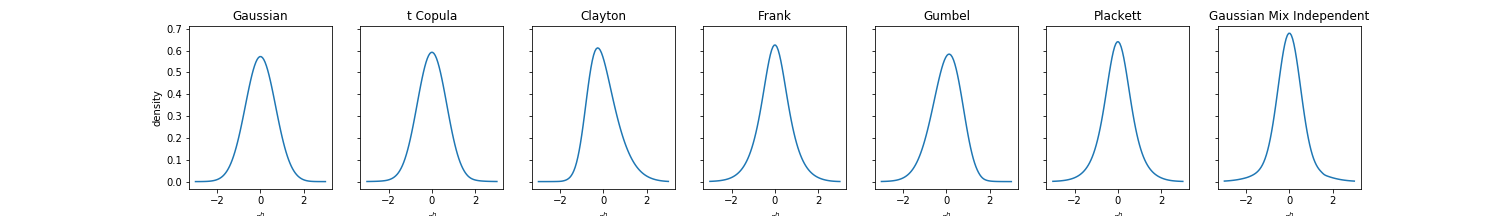
\includegraphics[width=\textwidth]{_pics/density illustration1.png}
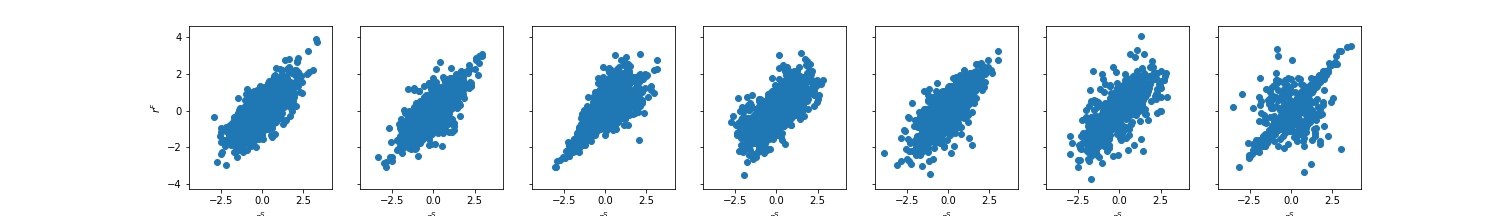
\includegraphics[width=\textwidth]{_pics/density illustration2.png}
  \caption{Upper Panel: Density of $Z= X - hY$ of different copulas with
  $X, Y \sim N(0,1)$,
  $0.75$ Spearman's rho between $X$ and $Y$, and $h=0.5$;
  Lower Panel: Scatter plot of samples from copulas.
  This illustration shows how dependence structure modelled by different copulas affects the density of the linear combination
  of margins.
  Notice that the $Z$ modelled by the asymmetric copulas, namely the Clayton and Gumbel copulas, are skewed to right
  and left respectively. \href{http://www.quantlet.com/}{
\includegraphics[width=15pt]{_pics/qletlogo_tr.png}}}
\label{fig:density illustration}
\end{figure}

%OLD
%\section{Methodology}\label{sec:methodology}
%Following \citet{barbi2014copula}, we consider the problem of optimal
%hedge ratios by extending the commonly known minimum variance hedge
%ratio to more general risk measures and dependence
%structures.\medskip
%
%Hedge portfolio: $R_t^h = R_t^S - h R_t^F$, involving returns of spot
%and future contract and where $h$ is the hedge ratio.\medskip
%
%The optimal hedge ratio is
%\begin{align}
%    h^\ast = \argmin_h \rho_\phi(s,h),
%    \end{align}
%for given
%confidence level $1-s$ (if applicable, e.g.\ in the case of VaR, ES),
%where $\rho_\phi$ is a spectral risk measure with weighting function
%$\phi$ (see below).
%In other words, our task is to search for the optimal $h$ which can minimize a particular risk measure.
%We call the risk measure being used in search process of $h^\ast$ risk reduction objective.
%This naming is to differentiate the risk objective and risk outcome.
%One can see from result section that the $h^\ast$ which minimize a particular risk measure in training does not
%necessarily minimize the risk measure in testing data.
%For example in table \ref{OOSRHVaR99}, the best performing risk reduction objective to reduce out-of-sample Value-at-Risk 99\% is
%exponential risk measure $k=10$. \medskip
%
%The distribution function of $R^h$ can be expressed in terms of the
%copula and the marginal distributions as Proposition \ref{prop:dfrh}
%result shows (this is a corrected version of Corollary 2.1 of
%\citep{barbi2014copula}). For practical applications, it is numerically
%faster and more stable to use additional information about the
%specific copula and marginal distributions. We therefore derive
%semi-analytic formulas for a number of special cases, such as the
%Gaussian-, Student $t$-, normal inverse Gaussian (NIG) and Archimedean
%copulas in Section \ref{sec:dependence}.
%
%\begin{proposition}
%  \label{prop:dfrh}
%  Let $R^S$ and $R^F$ be two real-valued random variables on the same
%  probability space $(\Omega, \mathcal A, p)$ with corresponding
%  absolutely continuous copula $C_{R^S, R^F}(w,\lambda)$ and
%  continuous marginals $F_{R^S}$ and $F_{R^F}$. Then, the distribution
%  of of $R^h$ is given by
%  \begin{equation}
%    \label{eq:3}
%    F_{R^h}(x) = 1- \int^1_0 D_1 C_{R^S, R^F}
%    \left( u, F_{R^F} \left( \frac{F^{-1}_{R^S}(u)-x}{h} \right)
%    \right)\, \dd u.
%  \end{equation}
%\end{proposition}\medskip
%Here $D_1 C(u,v)=\displaystyle \frac{\partial}{\partial u} C(u,v)$,
%which is easily shown to fulfil, see e.g.\ Equation (5.15) of
%\citep{McNeil2005}:\footnote{%
%  Let $F_X(x)=u$, $F_Y(y)=v$. Then, formally,
%  \begin{align*}
%    \frac{\partial}{\partial F_X(x)} C(F_X(x), F_Y(y)) %
%    &= \frac{\partial}{\partial F_X(x)} \p(U\leq F_X(x),
%      V\leq F_Y(y)) %
%      = \p(U\in \dd F_X(x), V\leq F_Y(y))\\ %
%    &= \p(V\leq F_Y(y)| U = F_X(x))\cdot \p(U \in \dd
%      F_X(x)) %
%      = \p(Y\leq y|X=x)\cdot \p(U\in \dd u)\\ %
%    &= \p(Y\leq y|X=x).
%  \end{align*}}
%\begin{equation}
%  \label{eq:1}
%  D_1 C_{X,Y}(F_X(x), F_Y(y)) = \p(Y\leq y|X=x).
%\end{equation}
%\begin{proof}
%  Using the identity (\ref{eq:1}) gives
%  \begin{align*}
%    F_{R^h}(x) &= \p(R^s - h R^F\leq x) %
%                 = \E\left[\p\left(R^F\geq \frac{R^S-x}{h}\Big|
%                 R^S\right)\right]\\[10pt]
%               &= 1-\E\left[\p\left(R^F\leq \frac{R^S-x}{h}\Big|
%                 R^S\right)\right]% \\[10pt]
%               = 1- \int_0^1 D_1 C_{R^S, R^F}\left(u,
%                 F_{R^F}\left(\frac{F^{(-1)}_{R^S}(u) -
%                 x}{h}\right)\right)\, \dd u.
%  \end{align*}
%\end{proof}\medskip
%
%In addition to \cite{barbi2014copula} we propose an expression for the density of $R^h$
%
%\begin{proposition} With the same setting of the above proposition, the density of $R^h$ can be written as
%  \begin{align}
%  f_{R^h}(y) &= \left|\frac{1}{h}\right|\int_0^1 c_{R^S, R^F} \left[u,
%  F_{R^F}\left\{\frac{F^{-1}_{R^S}(u)-y}{h}\right\}
%  \right]
%   \cdot
%  f_{R^F}
%  \left\{\frac{F^{-1}_{R^S}(u)-y}{h}\right\} du \label{eq:density1}
%  \end{align}, or
%    \begin{align}
%      f_{R^h}(y)
%      = \int_0^1 c_{R^S, R^F} \left[u,
%      F_{R^S}\left\{y + h F^{-1}_{R^F}(u)\right\}
%      \right]
%       \cdot
%      f_{R^S}
%      \left\{
%      y+ hF^{-1}_{R^F}(u)
%      \right\} du.\label{eq:density2}
%  \end{align}
%  \end{proposition}
